% 2015 年重庆卷（理工农医类）第 19 题：三棱锥 P-ABC，D 在 AB 上，E 在 BC 上（依固定扫描页重绘，只画拓扑与标号，不按比例）
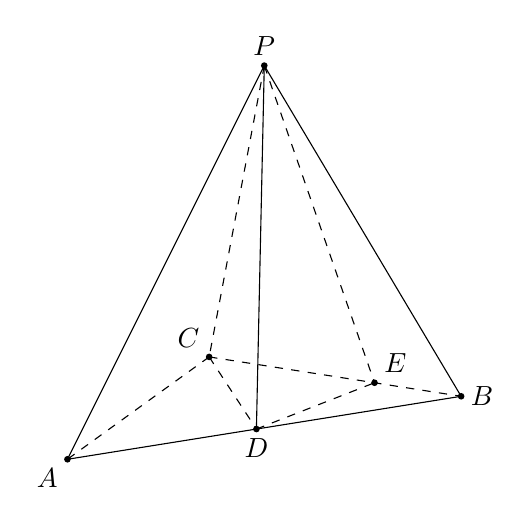
\begin{tikzpicture}[>=stealth,scale=1.0]
  % 顶点与底面各点
  \coordinate (P) at (4.0,6.0);
  \coordinate (A) at (1.5,1.0);
  \coordinate (C) at (3.3,2.3);
  \coordinate (B) at (6.5,1.8);
  \coordinate (D) at (3.9,1.384);
  \coordinate (E) at (5.4,1.972);
  % 实线棱
  \draw (P)--(A);
  \draw (P)--(B);
  \draw (P)--(D);
  \draw (A)--(B);
  % 虚线：PC、PE、CA、CB、CD、DE
  \draw[dashed] (P)--(C);
  \draw[dashed] (P)--(E);
  \draw[dashed] (C)--(A);
  \draw[dashed] (C)--(B);
  \draw[dashed] (C)--(D);
  \draw[dashed] (D)--(E);
  % 标号
  \fill (P) circle (1.2pt) node[above] {$P$};
  \fill (A) circle (1.2pt) node[below left] {$A$};
  \fill (B) circle (1.2pt) node[right] {$B$};
  \fill (C) circle (1.2pt) node[above left] {$C$};
  \fill (D) circle (1.2pt) node[below] {$D$};
  \fill (E) circle (1.2pt) node[above right] {$E$};
\end{tikzpicture}
